\documentclass[a4paper,oneside]{article}
\usepackage[utf8]{inputenc}
\usepackage{underscore}
\usepackage{setspace}
\usepackage{indentfirst} 
\usepackage{mathtools}
\usepackage{amsfonts}
\usepackage{enumitem}
% \usepackage[standard]{ntheorem}
\usepackage{amsthm}
\usepackage{cancel}
\usepackage{amssymb}
\usepackage[left=1.4cm,right=1.4cm,
    top=2.3cm,bottom=2.3cm,bindingoffset=0cm]{geometry}
\singlespacing

\usepackage{graphicx}
\graphicspath{ {./images/} }

\usepackage{fancyhdr}
\pagestyle{fancy}

\usepackage{tikz}
\usepackage[T2A]{fontenc}
\usepackage{graphicx}
\usepackage[sort,compress]{cite}
\usepackage{amsmath}
\usepackage{amssymb}
\usepackage{amsthm}
\usepackage{fancyvrb}
\usepackage{listings}
\usepackage{listingsutf8}
\usepackage{longtable}
\usepackage{array}
\usepackage[english,russian]{babel}
\usepackage{minted}
\usemintedstyle{xcode}

\usepackage[colorlinks=true]{hyperref}
\usepackage{url}
\usepackage{tempora}
\newcommand{\eqdef}{\stackrel {\rm def}{=}}

\usepackage{tabularx}
\newcommand{\bydef}{\stackrel{\text{по опр.}}{\implies}} % by definition - по определению
\newcommand{\parspace}{\vspace{10pt}}

\newcommand{\logor}{\vee}
\newcommand{\logand}{\wedge}

\newcommand{\imagin}{\mathrm{Im} \,}
\newcommand{\real}{\mathrm{Re} \,}

\newcommand{\dslim}{\displaystyle\lim}
\newcommand{\dslimn}{\dslim_{n \to \infty}}

\newcommand{\prop}[1]{#1^{\text{o}}}

\newcommand{\N}{\mathbb{N}}
\newcommand{\R}{\mathbb{R}}
\newcommand{\bb}[1]{\mathbb{#1}}

\newcommand{\eps}{\varepsilon}

\newcommand{\approach}[1]{\underset{#1}{\longrightarrow}}

% \theoremstyle{break}

% --- Теорема --- %
% \newtheoremstyle{break}% name
%   {}%         Space above, empty = `usual value'
%   {}%         Space below
%   {\itshape}% Body font
%   {}%         Indent amount (empty = no indent, \parindent = para indent)
%   {\bfseries}% Thm head font
%   {.}%        Punctuation after thm head
%   {\newline}% Space after thm head: \newline = linebreak
%   {}%         Thm head spec
% \theorembodyfont{\normalfont}
% \theoremstyle{break}
\newtheorem{theorem}{Теорема}[subsection]
% --------------- %

% --- Определение --- %
% \theorembodyfont{\normalfont}
\theoremstyle{definition}
\newtheorem{definition}{Определение}[subsection]
% ------------------- %

% --- Доказательство --- %
% \theoremheaderfont{\normalfont\itshape}
% \theorembodyfont{\normalfont}
% \newtheorem*{proof}{Доказательство.}
% ---------------------- %

% --- Пример --- %
\theoremstyle{definition}
\newtheorem*{example}{Пример}
% -------------- %

% --- Следствие --- %
% Corollary
% ----------------- %

% --- Замечание --- %
% Remark
\theoremstyle{definition}
\newtheorem*{remark}{Замечание}
% ----------------- %


\begin{document}

%----------------------------------------------------------------------------------------
%	TITLE PAGE
%----------------------------------------------------------------------------------------

\begin{titlepage} % Suppresses displaying the page number on the title page and the subsequent page counts as page 1
	\newcommand{\HRule}{\rule{\linewidth}{0.5mm}} % Defines a new command for horizontal lines, change thickness here
	
	\center % Centre everything on the page
	
	%------------------------------------------------
	%	Headings
	%------------------------------------------------
	
	\textsc{\LARGE Издательство Пупы и Лупы}\\[1.5cm] % Main heading such as the name of your university/college
	
	\textsc{\Large }\\[0.5cm] % Major heading such as course name
	
	\textsc{\large }\\[0.5cm] % Minor heading such as course title
	
	%------------------------------------------------
	%	Title
	%------------------------------------------------
	
	\HRule\\[0.4cm]
	
	{\huge\bfseries Лекции по лучшему языку на планете}\\[0.4cm] % Title of your document
	
	\HRule\\[1.5cm]
	
	%------------------------------------------------
	%	Author(s)
	%------------------------------------------------
	
	\begin{minipage}{0.4\textwidth}
		\begin{flushleft}
			\large
			\textit{Автор}\\
			\textsc{Пупа} % Your name
		\end{flushleft}
	\end{minipage}
	~
	\begin{minipage}{0.4\textwidth}
		\begin{flushright}
			\large
			\textit{Редактор}\\
			\textsc{Лупа} % Supervisor's name
		\end{flushright}
	\end{minipage}
	
	% If you don't want a supervisor, uncomment the two lines below and comment the code above
	%{\large\textit{Author}}\\
	%John \textsc{Smith} % Your name
	
	%------------------------------------------------
	%	Date
	%------------------------------------------------
	
	\vfill\vfill\vfill % Position the date 3/4 down the remaining page
	
	{\large\today} % Date, change the \today to a set date if you want to be precise
	
	%------------------------------------------------
	%	Logo
	%------------------------------------------------
	
	%\vfill\vfill
	%\includegraphics[width=0.2\textwidth]{placeholder.jpg}\\[1cm] % Include a department/university logo - this will require the graphicx package
	 
	%----------------------------------------------------------------------------------------
	
	\vfill % Push the date up 1/4 of the remaining page
	
\end{titlepage}

%----------------------------------------------------------------------------------------

\section{Теория множеств}

\subsection{Множества и отношения между ними}

Множество "--- совокупность различаемых объектов.
Объекты называются его элементами.

Два множества равны ($A = B$), если:

\begin{equation*}
     \forall x: (x \in A \Leftrightarrow x \in B)
\end{equation*}

Множество $A$ включается в множество $B$ ($A \subseteq B$), если:

\begin{equation*}
    \forall x: (x\in A \Rightarrow x \in B)
\end{equation*}

Множество, $A$ строго включается в множество $B$ ($A \subset B$), если:

\begin{equation*}
    \forall x: (A \subseteq B ~ \& ~ A \neq B)
\end{equation*}

Множество называется пустым, если оно не содержит элементов.
Такое множество обозначается как $\varnothing$.

\begin{equation*}
    \forall A \neq \varnothing: ~ \varnothing \subseteq A
\end{equation*}

Некоторое множество $\Omega \neq \varnothing$ назовем универсальным множеством
и скажем, что

\begin{equation*}
    \forall A \neq \varnothing: ~ A \subseteq \Omega
\end{equation*}

\subsection{Операции над множествами}

Пусть $A, B \subseteq \Omega$:

\begin{equation*}
    A \cup B = \{ \forall~ x\in \Omega: ~ x \in A \logor x \in B \} \quad \text{(объединение)}
\end{equation*}

\begin{equation*}
    A\cap B = \{ \forall ~ x \in \Omega: ~ x \in A \logand x \in B \} \quad \text{(пересечение)}
\end{equation*}

\begin{equation*}
    \overline{A} = \{ \forall ~ x \in \Omega: ~ x \notin A \} \quad \text{(дополнение)}
\end{equation*}

\begin{equation*}
    A \setminus B = \{ \forall ~ x \in \Omega: ~ x\in A \logand x \notin B \} = 
    A \cup \overline{B}  \quad \text{(разность)} 
\end{equation*}

\begin{equation*}
    A \triangle B = \{ \forall ~ x \in \Omega: ~ x\in A \logand x\notin B \logor x \notin A 
    \logand x \in B \} \quad \text{(симметричная разность)}
\end{equation*}

Множество, содержащее конечное число элементов называется конечным.

Пусть $ A \neq \varnothing$ и $A$ состоит из $n$ элементов, тогда $|A| = n$ "---
мощность этого множества.

Множество при этом также обозначается как $A = \{ a_1, a_2, \dots, a_n\}$ или $A = \{x ~|~ P(x) \}$

Примеры:

\begin{equation*}
    A = \{ x \in \R ~|~ x\geq 0 \logand x \leq 1 \}
\end{equation*}

\subsection{Характеристические векторы множеств}

Пусть есть некоторое конечное множество $\Omega \neq \varnothing$ из $n$ элементов, 
$\Omega = \{ x_1, x_2, \dots, x_n\}$

Для удобства будем считать, что порядок перечисления множеств зафиксирован.

Теперь пусть $A \subseteq \Omega$.

Характеристическим вектором $A$ назовем булев вектор из $n$ компонентов 

\begin{equation*}
    \chi_A = (\chi_1^A, \chi_2^A, \dots, \chi_n^A), \text{~где } \chi_i^A = 
    \begin{cases}
        1, & x_i \in A \\
        0, & x_i \notin A 
    \end{cases}
\end{equation*}

Пусть $P(A)$ "--- множество всех подмножеств непустого множества $A$. 

Отметим, что $A \in P(\Omega)$

Пример:

$\Omega = \{a, b, c\}$

$P(\Omega) = \{ \varnothing, \{a\}, \{b\}, \{c\}, \{a, b\}, \{b, c\}, \{a, c\}, \{a, b, c\} \}$
\begin{center}
    \begin{tabularx}{0.2\textwidth}{c|c}
        $A$ & $\chi_A$ \\ \hline
        $\varnothing$ & $(0, 0, 0)$ \\
        $\{ a \}$ & $(1, 0, 0)$ \\  
        $\{ b \}$ & $(0, 1, 0)$ \\  
        $\{ c \}$ & $(0, 0, 1)$ \\  
        $\{ a,b \}$ & $(1, 1, 0)$ \\  
        $\{ b,c \}$ & $(0, 1, 1)$ \\  
        $\{ a,c \}$ & $(1, 0, 1)$ \\  
        $\{ a,b,c \}$ & $(1, 1, 1)$ \\  
    \end{tabularx}    
\end{center}

Стоит отметить, что данное отображение является биективным. 

\begin{theorem}[о числе подмножеств конечного множества]
    Число подмножеств $n$"=элементного множества равно $2^n$:

    \begin{equation*}
        |P(\Omega)| = 2^n
    \end{equation*}
    
\end{theorem}

Двоичной алгеброй называется $B_2 = \{ 0, 1\}$ с операциями $\{', +, \cdot\}$, где


\begin{itemize}
    \item <<$'$>> "--- логическое <<НЕ>>
    \item <<$+$>> "--- логическое <<ИЛИ>>
    \item <<$\cdot$>> "--- логическое <<И>>
\end{itemize}


Обозначим $B_2^n$ множество всех двоичных векторов длины $n$.

Пусть $\vec{a} = (a_1, a_2, \dots, a_n), \vec{b} = (b_1, b_2, \dots, b_n) 
\in B_2^n$

\begin{enumerate}
    \item $\vec{a}' = (a_1', a_2', \dots, a_n')$
    \item $\vec{a} + \vec{b} = (a_1 + b_1, a_2 + b_2, \dots, a_n + b_n )$
    \item $\vec{a} \cdot \vec{b} = (a_1 \cdot b_1, a_2 \cdot b_2, \dots, a_n \cdot b_n)$
\end{enumerate}

\begin{theorem}[О характеристических векторах]
    Пусть $\Omega \neq \varnothing$ (универсальное множество).
    Для любых непустых множеств $A, B \subseteq \Omega$ справедливо следующее:
    \begin{enumerate}
        \item $A = B \iff \chi_A = \chi_B$
        \item $\chi_{A\cup B} = \chi_A + \chi_B$
        \item $\chi_{A\cap B} = \chi_A \cdot \chi_B$
        \item $\chi_{\overline{A}} = (\chi_A)'$
        \item $\chi_\varnothing = (0, 0, \dots, 0) = \vec{0}$
        \item $\chi_\Omega = (1, 1, \dots, 1) = \vec{1}$
    \end{enumerate} 
\end{theorem}

Пример:

\begin{example}
Пусть $\Omega = \{ 1, 2, 3, 4, 5\}$, $A = \{1, 3, 4\}$, $B = \{ 1, 4, 5\}$.

Тогда $\chi_A = (1, 0, 1, 1, 0)$, $\chi_B = (1, 0, 0, 1, 1)$.

Получим:

$\chi_{\overline{A}} = (0, 1, 0, 0, 1)$

$\chi_{A \cup B} = (1, 0, 0, 1, 0)$

$\chi_{A \cap B} = (1, 0, 1, 1, 1)$
\end{example}

\subsection{Декартово произведение и отношения между множествами}

Пусть $A, B \neq \varnothing$. Декартовым произведением множеств $A$ и $B$
назовем множество упорядоченных пар 

\begin{equation*}
    A \times B = \{ ~(a, b) ~|~ a \in A \logand b \in B\}
\end{equation*}

$(a_1, b_1) = (a_2, b_2) \iff a_1 = a_2 \logand b_1 = b_2$

Очевидно, что если $|A| = n$, $|B| = m$, то $|A\times B| = n \times m$. Кроме того, $|P(A\times B)| = 2^{nm}$

Бинарным отношением между множествами $A$ и $B$ назовем любое подмножество
декартового произведения $\rho \subseteq |A \times B|$.

Все теоретико"=множественные операции также справедливы для бинарных отношений.








    

\subsection{Разряды}

Шестнадцатиразрядные регистры DS ,ES, FS, GS, четыре сегментных регистра используются для определения начала сегментов данных.

CS "--- сегментный регистр сегмента кода, SS "--- сегмента стека.
Операционные системы могут размещать сегменты в ОП произвольным образом и даже временно записывать их на диск, если есть
нехватка оперативной памяти. Эти сегменты называются селекторами, они доступны программисту. 

С каждого сегмента есть программно-недоступный регистр называемый дескриптором. И в защищенном режиме именно в дескрипторе находится адрес
начала сегмента, его размер и некоторые другие аттрибуты. 

В реальном режиме, который чаще всего используется, размер
сегмента фиксирован, равен 64 Кбайтам, адрес сегмента кратен 16, поэтому в Шестнадцатиричной системе он записан
как 4 Шестнадцатиричные цифры и 0 (XXXX0).

В защищенном режиме размер может достигать до 4 Гбайт.

Всего сегментных регистров шесть, однако программист может в любой момент изменить содержимое сегментного регистра, таким
образом попасть в другой участок оперативной памяти. Например, если изменить содержимое регистра CS, процессор попадет
на выполнение другой программы "--- программы, содержащейся в другом участке памяти. Это может быть подпрограмма, либо
системно"=обрабатывающая программа.

Особенным образом реализуется SS. Адрес начала SS операционная система автоматически записывает в регистр SS. А указателем
на вершину стека является регистр SP "--- Stack Pointer, причем при добавлении элемента в стек содержимое регистра SP уменьшается.
Иными словами, стек растёт от максимально возможного значения вниз.

Такая реализация оказывается необходимой при работе с памятью в режиме flat, когда программа размещается в младших адресах
и с увеличением команды адреса растут, а стек размещается в старших адресах.

Если в стеке мы хотим хранить и фактические параметры, и локальные, то после загрузки фактических параметров в стек
указатель на вершину стека можно сохранять в специальном регистре Base Pointer(BP), И продолжая размещать локальные
параметры в стеке, мы сможем обращаться к фактическим параметрам, используя выражение $BP + k$, а к локальным $BP - r$,
где $k$ и $n$ "--- определяются количеством параметров и их размером.

Регистр flags определяет состояние программ и процессора в каждый текущий момент времени. Это 32-разрядный регистр, 
в котором 1, 3, 5, 15, 19-31 биты не используются. Девять флагов используются и в реальном, и в защищенном режиме,
следующие пять "--- только в защищенном режиме. Из девяти первых флагов шесть определяют состояние программы, а три определяют
состояние работы процессора. 

\begin{figure}[H]
    \centering
    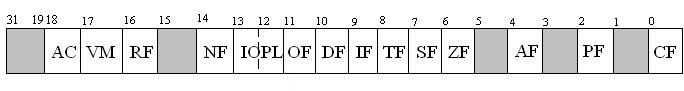
\includegraphics[scale = 0.5]{flags.jpg}
\end{figure}


\begin{enumerate}
\item CF "--- флаг переноса. Устанавливается в единицу, если при сложении происходит перенос за разрядную сетку, а при вычитании
требуется заём. 
\item FF "--- флаг четности. Устанавливается в единицу, если в младшем байте результата окажется четное количество единиц.
\item AF "--- флаг полупереноса. Устанавливается в единицу, если при сложении(вычитании) происходит перенос из третьего разряда
в четвертый(требуется заём из четвертого в третий)
\item ZF "--- флаг нуля. Устанавливается в единицу, если все разряды результата равны нулю.
\item SF "--- флаг знака. Всегда равен знаковому разряду результата. Положительный результат "--- ноль, отрицательный "--- единица.
\item TF "--- флаг трассировки. Установленный в единицу переводит процессор в режим пошагового выполнения программы.
\item IF "--- флаг прерывания. Установленный в единицу, позволяет остановить обработку некоторых прерываний.
\item DF "--- флаг направления. Определяет режим работы со строками. Если DF равен нулю, строка обрабатывается в сторону старших
адресов, в сторону младших в противном случае. При этом автоматически увеличивается(уменьшается) содержимое индексных регистров
если DF = 0 (DF = 1).
\item OF "--- флаг переполнения. Устанавливается в единицу, если результат превышает максимально допустимый для данной разрядной
сетки.
\item AC "--- флаг выравнивания операндов. Установленный в единицу, вызовет сообщение об ошибке, если адреса слов и двойных слов
не кратны двум или четырем соответственно.
\item VM "--- флаг виртуальных машин. Установленный в единицу, ползволяет перевести процессор в режим виртуальных машин.
\item RF "--- флаг маскирования прерывания. Позволяыет запретить прерывание.
\item NT "--- флаг вложенной задачи. Позволяет перейти в режим вложенной задачи.
\item IOPL "--- флаг уровня привелегий текущей программы. Если он окажется меньше значения флага, то программе будут запрещены
операции ввода/вывода.
\end{enumerate} 

\subsection{Оперативная память (RAM)}

Оперативная память состоит из байтов. Байт состоит из восьми информационных битов. Разряды с нулевого по третий "---
цифровая часть байта, с четвертого по седьмой "--- зонная часть байта.
\begin{figure}[H]
    \centering
    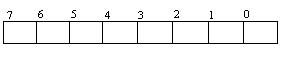
\includegraphics[scale = 0.5]{ram.jpg}
\end{figure}
32-х разрядный процессор может работать с оперативной памятью до 4 Гб, а значит физический адрес байта может изменяться от 
0 до $2^32 - 1$, что в Шестнадцатиричной системе записывается как $00000000 -> FFFFFFFF$.

Байты могут объединяться в поля фиксированной и переменной длины. Такие поля имеют собственные имена "--- слово (2 байта), двойное слово (4 байта).
Поле переменной длины может состоять из произвольного количества байтов. Адресом такого поля может быть адрес любого байта,
но это адрес младшего байта, входящего в поле.

Поле может использоваться как непрерывная память, либо сегментированная. В случае, если память сегментирована, то память
записывается как <сегмент>: <смещение>, а вычислено может быть по формуле ФА = АС + ИА, где АС - опредяется сегметным регистром,
а ИА "--- смещение сегмента, формируемое в команде и зависит от способа адрессации операнда.

В защищенном режиме программа может определять до 16383 сегментов размером до 4 Гб, и таким образом работать с 
64 ТБайтами виртуальной памяти.

Для реального режима адрес сегмента определяется сегментным регистром, и для получения 20-разрядного двоичного адреса
байта содержимое сегментного регистра, смещенного на 4 разряда влево прибавляют смещение (ИА).

\section{Работа с ассемблером}
\subsection{Форматы данных}

Процессор ix86 вместе с сопроцессором могут обрабатывать целые числа без знака, целые числа со знаком, действительные с плавающей
точкой, двоично-десятичные, символы, строки, указатели.
\paragraph{Целые числа.}

Целые двоичные без знака могут занимать байт, слово или двойное слово и принимать числа из диапазона 0-255, 0-65535, 0-4294967295
соответственно.
Целые числа со знаком так же могут занимать байт, слово или двойное слово, но представляются в дополнительном коде.

Дополнительнй код положительного числа совпадает с записью числа, а дополнительный код отрицательного числа может быть получен по
формуле $X = 10^n - |X|$.
Дополнительный код двоичного числа можно получить инверсией всех разрядов числа и добавление единицы к младшему разряду.

Вычитание в машине заменяется сложением уменьшаемого и доп. кодом вычитаемого числа. 
Действительные числа(числа с плавающей точкой) могут занимать 32 разряда (короткое), 64 разряда (длинное), 80 разрядов (рабочее).
Формат числа с плавающей точкой состоит из трех полей: знак числа, машинный порядок и мантисса.

Порядки:

$1 + 8 + 23 -> -10^{+-32} - 10^{+-32}$

$1 + 11 + 52$

$1 + 15+ 64$

Машинный порядок неявным образом включает в себя знак порядка. Он связан истинным следующим соотношением: $P_m = P_i + 127(1023, 16383)$.
Мантисса должна быть нормализованной, и старшая единица в разрядную сетку не помещается для экономии памяти.

\paragraph{Двоично"=десятичные числа.}

Процессор может обратаывать двоично"=десятичные числа в упакованном или неупакованном формате, а 
сопроцессором могут обрабатываться 90-ти разрядные данные в упакованном формате.

Они неупакованные "--- одну цифру в одной части байта.

\paragraph{Символы.}

Для символом используется кодировка ASCII. Для любого символа отводится один байт.
Строковые данные являются последовательностью байтов, слов или двойных слов.

Указатели на строку подразделяются на два типа:
длинный указатель, занимающий 48 бит (32 смещение + 16 сегмент)
короткий указатель, занимающий 32 бита(32 смещение)

\subsection{Форматы команд}

Команды "--- последовательность нулей или единиц, состоящих из двух подпоследовательностей.
Одна из них определяет код операции (сложить, умножить и т.~д), а другая определяет адреса операндов
и адрес размещения результата команды.

Операндами могут быть байтом, словом или двойным словом. Команда в свою очередь может быть безадресной, 
одноадресной, двухадресной или трехадресной.

В памяти команда может занимать от одного до 15 байтов, в зависимости от кода операции, количества и
размера операндов. Операнды могут находиться в команде, в регистрах или памяти. В одноадресной команде
операнд находится или в регистре, или в памяти, самое большое количество команд "--- двухадресные.

Существуют различные форматы двухадресных команд, которые отличаются расположением команд.
Регистр"=регистр, память"=память, регистр"=память, память"=регистр, данные"=память, память"=данные.

В общем случае, исполняемый адрес может состоять из трех частей: база, индекс и смещение.
Существуют различные способы способы адресации операндов, такие как:
\begin{enumerate}
    \item регистровая
    \item непосредственная
    \item прямая
    \item косвенно"=регистровая
    \item по базе со смещением
    \item прямая с индексированием
    \item по базе с индексированием (двумерные массивы)
    \item косвенная адресация с масштабированием
    \item базово"=индексная с масштабированием
    \item базово"=индексная с масштабированием и смещением
    
\end{enumerate}


\subsection{Примеры команд с различным способом адресации}

\begin{enumerate}
    \item Регистровая.
    \verb|mov AX, BX|
    \item Непосредственная.
    \verb|mov AX, 25|
    Кроме того, можно передать именованную константу с помощью конструкции \verb|const EQU 34h|
    \item Прямая. Если известен адрес в памяти, то в команде можно непосредственно передать этот адрес:
    \verb|mov AX, ES : 0001|, где ES "--- регистр сегмента данных, 0001 "--- смещение внутри сегмента. В таком случае
    содержимое двух байтов, начиная с адреса (ES) + 0001 пересылаются в AX
    ((ES) + 0001) -> AX

    Прямая адресация может быть записана с помощью символического имени, если этому имени
    предварительно поставить в соответствие некоторый адрес в оперативной памяти, а сделать
    это можно с помощью специальной директивы "--- директивы определения данных и памяти.
    
    DB "--- define byte
    DW "--- define word
    DD "--- define double word
    
    Если в сегменте ES содержится директива Var_p DW ?, тогда передадим по команде

    \verb|mov AX, ES: Var_p; ((ES) + Var_p) -> AX|
    \item Косвенно"=регистровая
    
    Данный вид адресации отличается от регистровой адресации тем, что в регистре содержится
    не сам операнд, а адрес области памяти, в которйо операнд содержится.
    
    \verb|mov AX,[SI]|
    
    Нельзя использовать AX, CX, DX, SP, ESP, остальные регистры допустимы.
    
    \item По базе со смещением

    \verb|mov AX, [BX] + 2; ((DS) + BX + 2)->AX|

    \verb|mov AX, [BP] + 4; ((SS) + (BP) + 4)->AX|
    
    \item Прямая с индексированием
    
    \verb|mov AX, MAS[SI]; ((DS) + (SI) + MAS)->AX|

    Эту адресацию используют с полями структуры. С двумерными массивами можно работать с адресацией по базе с индексированием.
    
    \item По базе с индексированием
    
    \verb|mov AX,Arr[BX][DI]; ((DS) + (BX) + (DI) + Arr)->AX|

    \item По базе с масштабированием
    
    \verb|MOVAX, [EBX*4]+2; Только для 32-х разрядных операндов|

Символическое имя определяет начало массива, с помощью базового регистра осуществляется
переход от одной строки к другой. Кроме того, используется при массивах структур.
   
\end{enumerate}

Особенности работы команд пересылки:
\begin{itemize}
    \item Нельзя пересылать из одной памяти в другую
    \item Нельзя пересылать информацию из одного сегментного регистра в другой.
    Если есть такая необходимость нужно воспользоваться регистром общего назначения или стеком
    для промежуточной пересылки.
    \item Нельзя пересылать непосредственный операнд в сегментный регистр. Если же такая
    необходимость есть "--- использовать регистр общего назначения.
    \item Нельзя командой mov изменять содержимое регистра CS.
    \item Данные в памяти хранятся в перевернутом виде, а в регистрах в нормальном
    виде, команда mov это учитывает.
    Например, R DW 1234h. Тогда в байте с адресом R будет 34h, а в байте R + 1 12h.
    Обратная картина в AH и AL при выполнении mov AX, R.
    \item Размер передаваемых данных определяется типом операнда.
    Например, пусть \verb|X DB ?, Y DW ?|, тогда при выполнении \verb|mov X, 0| в один байт запишется
    ноль, а если \verb|mov Y, 0| "--- два байта вместо одного.

    \verb|mov [SI], 0| "--- сообщение об ошибке. Чтобы этого не случилось, нужно определить
    тип операнда с помощью оператора PTR:

    \verb|<ТИП> PTR <ВЫРАЖЕНИЕ>|

    Выражение может быть как константным, так и адресным, а тип это: BYTE, WORD, DWORD и т.д.

    Например: \verb|mov Byte PTR[SI], 0| или \verb|mov [SI], byte PTR 0|.
    \item Если тип обоих операндов определен, известен, то эти типы должны соответствовать друг@=другу.
\end{itemize}

К командам пересылки относится команда \verb|xchg|. Операндами могут быть регистр"=регистр, регистр"=память.
Для перестановки значений байтов внутри регистра используют \verb|BSWOP|.

Также существуют команды конвертирования: \verb|CRW, CWD, CWE, CDF| (последние две для x386 и выше).

Есть команды условной пересылки: \verb|CMOVxx|.

Команда загрузки адреса: \verb|LEA OP1, OP2| "--- вычисляет адрес OP2 и пересылает первому операнду,
который может быть только регистром.

\subsection{Структура программы на ассемблере}

Программа на ассемблере должна пройти три этапа обработки.

На первом этапе, в процессе ассемблирования, исходный модуль преобразуется в машинный
код, таким образом получается объектный модуль исходных модулей и объектов может быть
несколько.

На втором этапе с помощью редактора связей (компоновщика) объектные модули преобразуются
в исполняемый модуль (\verb|.exe|, \verb|.com|). Для получения com"=файла нужно выполнить ещё один
этап обработки с помощью системной обрабатывающей программы. Для получения \verb|.com| файла
из \verb|.exe| файла нужно, чтобы исходный модуль удовлетворял определенным требованиям.

Исходный файл на ассемблере состоит из команд, директив и комментариев. Команды
в процессе ассемблирования преобразуются в программы на машинном языке, определяющим
этапы решения задачи. Директивы определяют форматы данных (исходных, промежуточных, окончательных)
и их размещение в памяти, а также определяют как программа должна быть транслирована ассемблером.

Команда в ассемблере в общем виде состоит из четырех полей:

\verb|[<имя>][:]<код операции>[<операнды>][комментарий]|

В скобках располагаются необязательные поля. Имя "--- символическое имя ассемблера, которое
используется как метка команды, на которую можно передать управление. Если после
имени стоит двоеточие, то такая метка называется внутренней и на нее можно передать
управление только из сегмента, в котором эта команда содержится.

Операнды отделяются друг от друга запятой, все поля отделяются друг от друга хотя бы
одним пробелом, а перед комментарием ещё записывается точка с запятой. Комментарий
может занимать часть строки или всю строку.
Например, \verb|JMP M1| "--- команда передачи управления на команду с меткой M1.

Директива, как и команда, состоит из четырех полей:

\verb|[<имя>]<код псевдооперации> <операнды> [; комментарий].|

Код псевдооперации  назначение директивы.
Операндов может быть различное количество в одной директиве.

\verb|M1 DB 1, 0, 1, 0, 1| "--- выделение пяти байтов подряд.

Proc "--- директива начала процедуры, endp "--- конца.

Исходный модуль на ассемблере состоит из последовательности строк, команд, директив и комментариев
и при ассемблировании текст просматривается сверху вниз слева направа от начала, пока
не увидит директиву end, которая и символизирует конец исходного текста программу.
Обычно программа состоит из трех сегментов. 

\begin{minted}{asm}
    Sseg Segment
    ...
    Sseg ends
    DSeg Segment
    ...
    DSeg ends
    CSeg Segment
    ...
    Cseg ends
    end start
\end{minted}

Каждый сегмент начинается с директивы Segment и заканчивается директивой ends. Параметры
директивы Segment говорят о назначении сегмента. Кроме того, в кодовом сегменте сразу
после директивы Segment должна располагаться директива, устанавливающая соответствие
между именами в директивах Segment и сегментными регистрами "--- \verb|assume|.

\begin{minted}{asm}
    assume SS :SSeg, CS: CSeg, DS: Dseg, ES: Dseg
\end{minted}

Кодовый сегмент выглядит как процедура, это может быть одна процедура или последовательность
процедур.

Структура кодового сегмента с использованием двух вложенных процедур выглядит следующим
образом:

\begin{minted}{asm}
    Cseg segment...
    assume...

    pr2 Proc
    ...
    pr2 ends

    pr1 Proc
    ...
    pr2
    pr1 ends

    end pr1
\end{minted}

В сегменте стека выделяется место под стек.
В сегменте данных определяются данные, используемые в программе, выделяется место
под промежуточные и окончательные результаты.
Кодовый сегмент содержит программу решения поставленной задачи.

\begin{minted}{asm}
    ;Prim1.asm
    ;Сегмент стека
    Sseg segment
        db 256 dup(?)
    Sseg ends
    ;Сегмент данных
    Dseg segment
        X db 'A'
        Y db 'B'
        Z db 'C'
    Dseg ends
    Cseg segment
        assume SS:Sseg, DS:DSeg, CS:Cseg
        start proc FAR
        push DS
        push AX
        mov DS, Dseg
        mov DS, DX
        call Main
        ret
    Start endp
    main proc NEAR
        add AL, X
        mov AX, Y
        ...
        ret
    main endp
    Cseg ends
    end start
\end{minted}

Наш кодовый сегмент представлен в виде двух последовательных процедур: первая из них
внешняя, об этом говорит параметр \verb|far| директивы \verb|Proc|, она реализует связь с операционной системой.
\verb|near| же говорит о том, что процедура внутренняя.

К внешней процедуре можно обратиться из любого кодового сегмента, к внутренней можно обратиться
только из того сегмента, в котором содержится её определение.

Программа на ассемблере может работать с целыми двоичными, десятичными, шестнадцатиричными, действительными
с плавающей точкой числами, символами и строками. Сигнатура двоичных чисел имеет вид <<xxxxb>>.

Десятичная константа записывается как обычное число, а шестнадцатиричная содержать <<h>> на конце,
если же ведущая цифра это А, B, C, D, E, F, то в начале необходимо поставить 0.

Двоичные числа имеют вид мантисса"=порядок. 

Пример: 34,751e+02. 

Строковые константы "--- последовательности символов,
заключенных апострофами или двойными кавычками.

Как и в языках высокого уровня, на ассемблере могут быть именованные или неименованные константы.
Примеры неименованных были рассмотрены выше, их тип и значение определяются внешним видом на этапе компиляции.
Именованные константы создает программист с помощью специальной директивы EQU. Пример: M EQU 27.
Символическому имени M присваивается константное значение 27.

Переменные в ассемблере определяются с помощью директивы определения данных и памяти: v1 DR ?
v2 DW 34 или с помощью знака равенства: v3 = 100. 
Константы обычно используются как непосредственный операнд и в директивах определения данных и памяти.

Выражения в ассемблере строятся из операндов, операторов и скобок. Операнды "--- константы и переменные,
операторы "--- знаки арифметических, логический, специальных операций, а также операций отношения.
Все арифметические, логические операции и операции отношения характерны и другим языкам. Среди специальных
операций выделяют offset и PTR. offset возвращает смещение переменной относительно начала сегмента.
PTR определяет один из следующих типов для операнда:
\begin{itemize}
    \item BYTE
    \item WORD
    \item DWORD
    \item FWORD
    \item QWORD
    \item TWORD  
\end{itemize}
Кроме того, к специальным операциям относят \verb|near| и \verb|far|.

\subsubsection{Директива определения.} 
Её синтаксис следующий:

\verb|[<имя>] D{X} <операнды>[<;комментарий>], где X "--- B, W, D, F, Q, T.|

Имя определяет адрес первого байта выделенного поля (если оно есть), операндом может быть знак вопроса
или константа. Если это константа, то она записывается в выделенное поле, если знак вопроса, то в выделенное поле не записывается ничего.

Если операндом является символоическое имя (пусть это будет \verb|IM1|), которому предварительно поставлено
в соответствие некоторое значение, например, \verb|03AC1h|, то после выполнения
\verb|M DD IM1| будет выделено 4 байта памяти, в которое запишется значение \verb|03AC1h|.

Для выделения большого количества памяти используются директива \verb|dup|, например \verb|D db 100 dup (1)|.
Аналогично определяется, например, одномерный массив слов, например \verb|mas dw 1, 7, 35, 75, 84|.
У двумерного массива хранится указатель на элемент нулевой строки, нулевого столбца.

\begin{minted}{asm}
    const EQU 100
    d db const dup (?)    
\end{minted}


C помощью директивы определения байта возможно определить константу максимальной допустимой величины 255, для слова "--- 65535.

С помощью директивы определения байта можно определить строковую константу до 255 символов

Команда прерывания.

Команда прерывания приостанавливает выполнение программы и передает выполнение операционной системе
или BIOS в зависимости от операнда этой команды, после чего выполняется системная обрабатывающая программа
и управление возвращается к следующей за ним. А какая системная обрабатывающая программа будет выполняться
зависит от содержимого некоторых регистров. Например: чтобы вывести на экран символ, нужно выполнить три команды:
\begin{minted}{asm}
    mov AH, 6
    mov DL, "!"
    int 21h    
\end{minted}
Стек определяется регистрами SS и SP(ESP).
Начало сегмента стека записывается в регистр SS автоматически, 
а указатель на вершину стека при добавлении элемента уменьшается на размер операнда, при удалении
"--- увеличивается. Чтобы добавить элемент в стек нужно вызвать функцию push, чтобы удалить "--- pop.

Для i186 существуют команды \verb|pusha| И \verb|popa|, которые позволяют загрузить и удалить последовательность регистров
AX, BX, DX, CX, SP, BP, SL, DL. С i386 есть команды pushad и popad "--- аналогичные команды для extended версий
регистров.

\begin{minted}{asm}
TITLE Pris.asm; заголовок листинга
Page, 120; длина
SSeg Segment Para stack 'stack'
DB 100h
SSeg ends

DSeg Segment Para Public 'Data'
DAN DB '1', '3', '5', '7'
REZ DB 4 DUP (?)
DSeg ends
;кодовый сегмент оформлен как одна внешняя процедура, к ней обращаются из отладчика

CSeg Segment Para Public 'Code'
ASSUME SS:SSeg, DS:DSeg, CS:CSeg; соответствие между сегментными регистрами и именами
start proc Far
push DSeg
xor AX, AX
push AX
mov AX, DSeg
mov DS,AX
mov AH, 6
mov DL, DAN + 3
mov REZ, DL
int 21h
mov DL, DAN + 2
mov REZ + 1, DL
int 21h
mov DL, DAN + 1
mov REZ + 2, DL
int 21h
mov DL, DAN
mov REZ + 3, DL
int 21h

mov AH, 4CH
int 21h
Start endp
CSeg ends
end Start
\end{minted}


\subsubsection{Директива сегмента.}

Общий вид:

\verb|<имя> Segment <ReadOnly> <Выравнивание> <тип> <размер> <'класс'>|.

\verb|ReadOnly| устанавливает режим только для чтения для этого сегмента.

Операнд <<выравнивание>> устанавливает адрес начала сегмента:
\verb|BYTE, WORD, DWORD| "--- кратность байту, двум или четырем соответственно.

\verb|Para| "--- кратность шестнадцати. \verb|Page| "--- кратность 256.

<<Тип>> определяет тип объединения сегментов. Для стека устанавливается stack, для остальных сегментов public.
Если этот параметр присутствует, то все сегменты с одним именем и различными кклассами объединяются в один
последовательно в порядке их записи.

Значение 'Common' говорит, что сегменты с одним именем объединены, но не последовательно, а с одного и того же
адреса так, что общий размер сегмента равен не сумме, а максимальному из них.

Значение \verb|IT <выражение>| означает, что сегмент должен быть расположен по абсолютному адресу, определяемым выражением.
'Private' говорит о том, что этот сегмент не объединяется ни с каким другим.

Параметр размер может принимать значения \verb|use 16|, \verb|use 32|.
\subsubsection{Точечные директивы.}

В программе на ассемблере могут использоваться точечные директивы:
.MODEL "--- директива, определяющая модель выделяемой памяти для программы.
МОдель памяти определяется параметром:
tiny "--- под всю программу выделяется 1 сегмент памяти.
small "--- под данный и под программу выделяются по одному сегменту.
medium "--- под данные выделяется один сегмент, под программу выделяется несколько сегментов.
compact "--- под программу выделяется один сегмент, под данные выделяется несколько сегментов.
large "--- под данные и под программу выделяются по n элементов.
huge "--- позволяет использовать сегментов больше, чем позволяет оперативная память.

\begin{minted}{asm}
    .model small
    .stack 100h
    .data 
    \dots
    .code
    begin:
    mov AX, @data
    mov ds, AX
    mov AH, 9
    mov DX, offset St1
    int 21h
    аналогично для остальных двух
    mov AH, 4CH
    int 21
    end begin    
\end{minted}

\subsubsection{COM"=файлы}

Результатом ассемблирования и редактора"=компоновщника является исполняемый exe"=файл, которые содержит в себе,
так называемый, блок начала загрузки размером в 512 байт.

Но ассемблер позволяет создать другой тип исполняемых
файлов \verb|.com|, который может быть получен на основе \verb|.exe| файла в результате его обработки системной программой
\verb|EXE2bin.com| или с помощью специального ключа в среде разработки. 
Не из всякого EXE"=файла можно создать
COM"=файл "--- исходный файл должен удовлетворять определенным требованиям.

\paragraph{Основные отличия}
\begin{itemize}
    \item COM"=файл не содержит блока начальной загрузки(512 байт)
    \item EXE"=файл занимает произвольный объем ОП, COM"=файл только один сегмент памяти.
    \item в COM"=файле стек создается автоматически ОС, поэтому у пользователя нет необходимости выделять для него место.
    \item В COM"=файле данные располагаются там же, где и программа. Т.к вся программа содержится в одном сегменте, все сегментые регистры содержать
    в качестве значения адрес префикса программного сегмента (psp). И т.к PSP содержит 256 байт, то ддя обхода этого блока применяется org 100h.
\end{itemize})

\subsubsection{Арифметические операции}

\paragraph{Сложение и вычитание}
Сложение(вычитание) беззнаковых чисел выполняется по правилам аналогичным сложению (вычитанию)
по модулю $2^k$, принятым в математике. Если в результате более $k$ разрядов, то $k+1$"=ый пересылается
в \verb|CF|.

То есть:
\begin{equation*}
    \begin{cases}
        X + Y = (X + Y) \text{mod} ~2^k = X + Y, ~\text{CF} = 0 & \text{если $X + Y < 2^k$} \\
        X + Y = (X + Y) \text{mod} ~2^k = X + Y, ~\text{CF} = 1 & \text{если $X + Y \ge 2^k$} \\

    \end{cases}    
\end{equation*}

Пример:
\begin{equation*}
    250 + 10 = (250 + 10) ~\text{mod}~ 2^8 = 260~ \text{mod} ~256 = 4
\end{equation*}

Сложение (вычитание) знаковых чисел сводится к сложению (вычитанию) с использованием дополнительного кода.

Например, $-1 = 256 - 1 = 255 = {11111111}_2$, $-3 = 256 - 3 = 253 = {11111101}_2$
\begin{equation*}
    3 - 1 = 3 + (-1) = (3 + (-1))~\text{mod}~256 = (3 + 255)~ \text{mod}~256 = 2
\end{equation*}

Ответ получили в дополнительном коде, следовательно результат получаем  в байте по формуле $X = 10^8 - |X|$, т.~е.
$X = 256 - 254 = |2|$ и знак минус. Ответ: -2.

Переполнение разрядной сетки происходит если есть перенос из старшего цифрового в знаковый, а из знакового нет, и
наоборот, тогда OF = 1. Программист сам решает какой флажок анализировать "--- OF или CF, зная 
с какими данными он работает.

\paragraph{Сложение и вычитание в Ассемблере}

Арифметические операции изменяют значение флажков OF, CF, SF, ZF, AF, IF.

В Ассемблере операция сложения представлена несколькими командами.

\begin{minted}{asm}
    add OP1, OP2; (OP1) + (OP2) -> OP1
    adc OP1, OP2; (OP1) + (OP2) + (CF) -> OP1
    xadd OP1, OP2; (OP1)<->(OP2), (OP1) + (OP2) -> OP1
    inc OP1; OP1 + 1 -> OP1
\end{minted}

Аналогично работают команды sub, sbb, dec. В командах сложения (вычитания) можно использовать любые способы адресации.

\paragraph{Умножение и деление}

Умножение беззнаковых чисел представлено командой MUL.
\begin{minted}{asm}
    MUL OP2; (OP)*(AL) or (AX) or (EAX) -> AX or DX:AX or EDX:EAX
\end{minted}

Умножение знаковых чисел определяется аналогичным образом, но с помощью команды IMUL.




К командам побитовой обработки данных относятся логические команды, команды сдвига, установки, сброса и инверсии битов.

К логическим операциям относят команды and, or, xor, not. Для всех логических команд, кроме not операнды одновременно
не могут находится в памяти. OF = CF = 0, AF - не определен, SF, ZF, PF определяются результатом команды.

Второй операнд называют маской. Основным назначением команды and является установка в ноль с помощью маски
некоторых разрядов первого операнда. 

\subsubsection{Директивы внешних ссылок}

Директивы внешних ссылок позволяют организовать связь между различными модулями и файлами, расположенными на диске.

\begin{minted}{asm}
    Public <имя> [,<имя>, ..., <имя>]
\end{minted}

определяет указанные имена как глобальные аеличины, к которым можно обратиться из других модулей. Имена здесь "---
имена меток и переменных, определенных с помощью директивы '=' и EQU.

Если некоторое имя определено в модуле A как глобальное, и к нему можно обратиться из других модулей B и C, то в этих
модулях должна быть директива вида

\begin{minted}{asm}
    EXTRN <имя>:<тип> [,<имя>:<тип>]
\end{minted}
Здесь имя то же, что и в \textbf{Public}, а тип определяется
следующим образом: если <имя> "--- это имя переменной, то типом
может быть: BYTE, WORD, DWORD, FWORD, QWORD, TWORD.
Если <имя> "--- это имя метки, то типом может быть \textbf{NEAR} и \textbf{FAR}.

Директива \textbf{EXTRN} говорит о том, что перечисленные имена являются
внешними для данного модуля.

\subsubsection{Команды управления}


Передача параметров по ссылке

Оформим как процедуру вычисление $x = x div 16$

Процедура имеет один параметр-переменую x, которой в теле
процедуры присваивается новое значение. Т. е результат записывается
в некоторую ячейку памяти. И чтобы обратиться к процедуре с различными параметрами, например, a и b, ...


Процедура:

\begin{minted}{asm}
Proc_dv proc
	push CX
	mov CL, 4
	shr word ptr [BX], CL
	pop CX
	ret
Proc_dv endp
\end{minted}

Сдвиг на 4 разряда вправо эквивалентен делению нацело на шестнадцать.

При этом сохраняется содержимое регистра CX, т.к это значение перезаписывается в 4 строчке.

Т.к регистров немного, а ПП и основная программа могут использовать те же регистры, то при входе в ПП нужно сохранять все регистры, которые в этой подпрограмме используются, а перед выходом их восстанавливать. Именно для этой цели были введены команды, позволяющие сохранять все регистры общего назначения - $pusha$, $popa$, а .386 $pushad$, $popad$. Конечно, не нужно сохранять в стеке значения регистров, в которые записывается результат работы подпрограммы.

Передача параметров по ссылке в блоке параметров

Если параметров много, например, массив, адрес начала массива как блока параметров, можно передать через регистр, даже если результат ПП не будет записываться по этому адресу.

Пример:

Даны два массива целых положительных чисел без знака:
X DB 100 dup (?)
Y DB 50 dup (?)

Вычислить: DL = max(X[i]) + max(Y[I]), использовав процедуру max(A[i]), пересылая адрес массива через регистр BX,	а результат сохраняя в AL.

\begin{minted}{asm}
 lea BX, X
 mov CX, 100
 call max
 mov DL, AL
 lea BX, y
 mov CX, 50
 call max
 add DL, AL
 
 max proc
 push CX
 push BX
 mov AL, 0
 
 met1:
 cmp [BX], AL
 jle met2
 mov AL, [BX]
 
 met2:
 inc bx
 loop met1
 pop BX
 popCX
 ret
 max endp
\end{minted}

Передача параметров через стек

Этот способ передачи параметров называют универсальным, его можно использовать при любом количестве параметров, хотя он сложнее, чем передача параметров через регистры.

Если ПП имеет k параметров PP($a_1$, $a_2$ ... , $a_n$) размером в слово и параметры сохраняются в стеке в последовательности слева направо, то команды, реализующие обращение к ПП, должны быть следующими:

\begin{minted}{asm}
push a1
push a2
...
push ak
call PP
\end{minted}

В случае такого обращение содержимое стека в подпрограмме можно представить так

\begin{figure}[H]
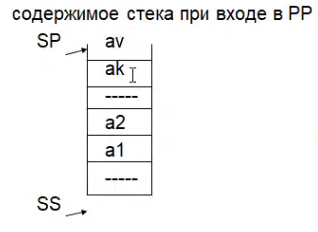
\includegraphics{prccstack.png}
\end{figure}

Обращение к параметрам в процедуре можно осуществлять с помощью значения BP, присвоив ему значение SP.

При этом мы испортим старое значение BP, которое могло быть использовано в основном программе. Поэтому следует в начале сохранить старое значение BP в стеке, а затем использовать его для доступа к параметрам, т.е тело процедуры должно начинаться следующими командами:

\begin{minted}{asm}
PP proc near
push BP
mov BP, SP
\end{minted}

\begin{figure}[H]
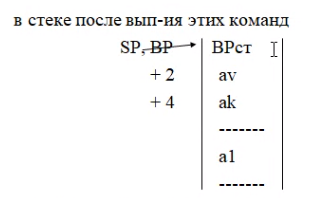
\includegraphics{procstack2.png}
\end{figure}

Для доступа к последнему параметру можно использовать выражение [BP + 4], например, mov AX, [BP + 4]; ak -> AX

После входных действий в ПП идут команды, реализующие вспомогательный алгоритм, а за ними д.б. команды, реализующие выходные действия.

\begin{minted}{asm}
pop BP
ret 2 * k
PP endp
\end{minted}

и в команде ret n - это количество освобождаемых байтов в стеке, поэтому количество д.б множено на длину параметра.

Команда ret вначале считывает значение ay, а затем удаляет из стека параметры. Очистку стека можно выполнять и не в ПП, а после выхода из нее, сразу после команды call PP, например, командой add SP, 2 * k.

Каждый способ имеет свои достоинства и недостатки.

Например, очищение в ПП позволяет сделать исполняемый код короче, а очищение в основной программе позволяет вызвать ПП несколько раз с одними и теми же параметрами последовательностями команд call.

для удобства использования параметров, переданных через стек, внутри ПП можно использовать директиву equ, чтобы при каждом обращении к параметрам не писать точное смещение относительно BP.

Пример:

push x
push y
push z
call PP

\begin{minted}{asm}
PP proc near
push BP
mov BP, SP
pp_x equ[BP + 8]
pp_y equ[BP + 6]
pp_z equ [BP + 4]

mov AX, pp_x

pop BP
ret 6
PP endp
\end{minted}

Пример передачи параметров через стек.

Пусть процедура заполняет нулями массив A[0, n - 1], а основная программа обращается к ней для обнуления массивов X[0..99] и Y[0..49]. Через стек в ПП передается имя массива и его размер, размер можно передавать по значению, а имя массива нужно передавать по ссылке, т.к этот параметр является и входным, и выходным.

\begin{minted}{asm}
zero_1 proc
push BP
mov BP. SP
push BX
push CX
mov CX, [BP + 4]
mov BX, [BP + 6]
mov byte ptr [BX], 0
inc BX
loop m1
pop CX
pop BX
pop BP
ret 4
zero_1 endp

Main:

x DB 100 dup (?)
y DB 50 dup (?)

lea AX, x
push AX
mov AX, 100
push AX
call zero_1
lea AX, y
push AX
mov AX, 50
push AX
call zero_1

end Main
\end{minted}

О передаче параметров в ПП

\begin{itemize}
\item Передача по значению
mov AX, word ptr value
\item Передача по ссылке
mov AX, offset value
call PP
\item Передача параметров по возвращаемому значению объединяет передачу по значению и по ссылке: процедура передается адрес переменной, она делает локальную копию этого параметра, работа с этой компией, а в конце процедуры записывает эту копию по переданному адресу. Этот механизм оказывается эффективным, если процедуре приходится много раз обращаться к параметру в глобальной переменной.
\item Передача параметров по результату заключатеся в том, что ПП передается адрес только для записи по этому адресму результата работы ПП.
\item Передача параметров по имени макроопределения
name macro parametr
mov AX, parametr
name endm
Обращение к ПП может быть таким:
name value
call PP
\item Передача параметров отложенным вычислением. Как и в случае передачи параметров по имени макроса, процедура получает адрес ПП, вычисляющей значение параметра. Этот механизм чаще используется в системах искусственного интеллекта и в ОС.
\end{itemize}

Использование локальных параметров.

Если локальных параметров немного, то их размещают в регистрах, но если их много, возможны различные варианты: им можно отвести место в сегменте данных, но тогда большую часть времени эта память не будет использоваться.

Лучший способ - разместить локальные переменные в стеке на время работы ПП, а после выхода из ПП их удалить. для этого после входных действий в процедуре нужно уменьшить значение указателя на вершину стека SP на количество байтов, необходимых для хранения локальных величин и затем записывать их в стек и извлекать можно с помощью выражений вида:

[BP - n], где n определяет смещение локального параметра относительно значения BP.

Например, если предполагается, что ПП будет использовать 3 локальных параметра размером в слово, то стек графически можно представить так:

\begin{figure}[H]
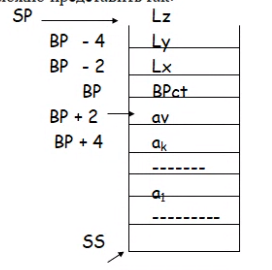
\includegraphics{procstack3.png}
\end{figure}

При выходе из процедуры перед выполнением завершающих действий нужно вернуть регистру SP его значение.

Если в стеке хранятся и фактически, и локальные параметры, то начало процедуры и её завершение должно выглядеть следующим образом:

\begin{minted}{asm}
PP proc
push BP
mov BP, SP
sub SP, k1
push AX; сохраняем в стеке регистры, используемые в ПП
----------
<тело процедуры>
-----------
pop AX ; восстанавливаем регистры
mov SP, BP; освобождаем место в стеке от локальных параметров
pop BP; восстанавливаем BP
ret k2; очищаем стек от фактических параметров
pp endp
\end{minted}

Подсчет количества различных символов в заданной строке

Строка задана как массив символов. начальный адрес ее передадим в ПП через регистр BX, длину строки через CX, а результат - через AX. Создадим процедуру, в которой выделяется 256 - байтный локальный массив L по количеству возможных символов. K - му элемент этого массива будем присваивать единицу, если символ, цифровой код которого равен К, в заданной строке существует. 

Затем подсчитаем количество единиц в этом массиве. Вначале весь массив обнуляется. К первому элементу этого массива можно обратиться так:

$L_1 = [BP - 256]$ к К - му, $L_k = [BP - 256 + k]$

Работая со строками, эту задачу можно решить проще.

\begin{minted}{asm}
count_s proc
push BP
mov BP, SP
sub SP, 256
push BX
push CX
push SI
mov AX, CX
mov CX, 256
mov SI, 0
m1:
mov byte ptr[BP - 256 + SI], 0
inc SI
loop m1

mov CX, AX
mov AX, 0
m2:
mov AL, [BX]
mov SL, AX
mov byte ptr[BP - 256 + SI], 1
inc BX
loop m2
mov AX, 0
mov CX, 256
mov SI, 0
m3:
cmp byte ptr[BP - 256 + SI], 1
jne m4
inc AX
m4:
inc SI
loop m3
pop SI
pop CX
pop BX
mov SP, BP
pop BP
ret
count_s endp
\end{minted}

Рекурсия в Ассемблере



\section{Работа с программами}

Программа, оформленная как процедура, к которой обращение происходит из ОС, заканчивается командой возврата ret.

Подпрограмма, как вспомогательный алгоритм, к которому возможно многократное обращение с помощью команды call,
тоже оформляется как процедура с помощью директив proc и endp. Структуру процедуры можно оформить так:

\begin{minted}{asm}
    <имя процедуры> proc <параметр>
        <тело процедуры>
        ret
    <имя процедуры> endp
\end{minted}

В Ассемблере один тип подпрограмм - процедура. Размешать ее можно в любом месте программы, но так, чтобы управление на нее не попадало случайно, а только по команда call.
Поэтому описание ПП принято располагать в конце программного сегмента (после последней исполняемой команды), или вначале его - перед первой исполняемой командой.

\section{Графическое представление}

\begin{minted}{asm}
    1) cseg segment .....
    beg: ----------------
    ---------------------
    ---------------------
    fin: ----------------
    <подпрограмма 1>
    <подпрограмма 2>
    ---------------------
    <подпрограмма n>
    cseg ends
    end beg
\end{minted}

\begin{minted}{asm}
    2) cseg segment
    <подпрограмма 1>
    <подпрограмма 2>
    ---------------------
    <подпрограмма n>
    beg:-----------------
    ---------------------

    cseg ends
    end beg
\end{minted}

\begin{minted}{asm}
    3) cseg_pp segment
    <>
    cseg_pp ends
    cseg segment...
    ---------------------
    cseg ends
    end beg
\end{minted}

Если программа содержит большое количество подпрограмм, то ПП размещают в отдельном кодовом сегменте - вариант структуры 3).

\paragraph{Замечания:}

\begin{itemize}
    \item После имени в директивах proc и endp двоеточие не ставится, но имя считается меткой, адресом первой исполняемой процедуры.
    \item Метки, описанные в ПП, не локализируются в ней, поэтому они должны быть уникальными в рамках всей программы.
    \item Параметр в директиве начала процедуры один - FAR или NEAR.
\end{itemize}

Основной проблемой при работе с ПП является передача параметров и возврат результатов в вызывающую программу.
Существуют различные способы передачи параметров:
\begin{enumerate}
    \item по значению;
    \item по ссылке;
    \item по возращаемому значению;
    \item по результату;
    \item отложенным вычислением.
\end{enumerate}

Параметры можно передавать:
\begin{enumerate}
    \item через регистры;
    \item в глобальных переменных;
    \item через стек;
    \item в потоке кода;
    \item в блоке параметров.
\end{enumerate}

Передача параметров через регистры - наиболее простой способ. Вызывающая программа записывает в некоторые регистры фактические парамтеры...

\textbf{Примерами использования этого метода являются вызовы некоторых прерываний ОС и BIOS.}

Когда регистров не хватает, один из способов обойти это ограничение - записать параметр в глобальную переменную, к которой затем обращаться в ПП.
Но этот мето считается не эффективным, так как может оказаться невозможной рекурсия, и даже простое повторное обращение к ПП.

Передача параметров через стек. Перед обращением к процедуре фактические параметры (их значения или адреса) записываются в стек, а процедура их из стека извлекает.
Именно этот способ используют языки высокого уровня.

Передача параметров в потоке кода заключается в том, что данные, передаваемые в ПП, располагаются сразу за командой обращения к ПП call.
ПП, чтобы использовать эти данные, должна обратиться к ним по адресу, который записывается в стек автоматически как адрес возврата из ПП.
Но ПП в этом случае должна перед командой возврата изменить адрес возврата на адрес байта, следующий за передаваемыми параметрами. Этот метод реализует передачу
параметров медленнее, чем через регистры, глобальные переменные или стек, но примерно также, как и метод передачи параметров в блок параметров.

Блок параметров - это участок памяти, содержащий параметры и располагающийся обычно в сегменте данных.

Процедура получает адрес начала этого блока при помощи любого из рассмотренных методов: в регистре, в переменной, в стеке, в коде или даже в другом блоке параметров.
Примеры использования этого способа - многие функции ОС и BIOS, например, поиск файла, использующий блок параметров DTA, или загрущка и исполнение программы, использующая блок параметров EPB.

\subsection{Передача параметров по значению и по ссылке}

При передаче параметров по значению процедуры передается значение фактического параметра, оно копируется в ПП, и ПП использует копию, поэтому изменение, модификация параметра
оказывается невозможным. Этот механизм используется для передачи параметров небольшого размера.

Например, нужно вычислить \textbf{c = max(a, b) + max(7, a-1)}. Здесь все числа знаковые, размером в слово. Используем передачу параметров через регистры. Процедура получает параметры через
регистры. Процедура получает параметры через регистры AX и BX, результат возвращается в регистр AX.
Процедура:
\begin{minted}{asm}
    AX = max(AX, BX)
    max proc
        cmp AX, BX
        jge met1
        mov AX, BX
        met1: ret
    max endp
\end{minted}

\section{Фрагмент вызывающей программы:}
-----------------
\begin{minted}{asm}
    ; c = max(a, b) + max(7, a-1)
    mov AX, a
    mov BX, b
    call max ; AX = max(a, b)
    mov c, AX ; c = max(a, b)
    mov AX, 7
    mov BX, a
    dec BX
    call max ; AX = max(7, a-1)
    add c, AX
\end{minted}
-----------------

\section{Передача параметров по ссылке.}

Оформим как процедуру вычисление \textbf{x = x div 16}

Процедура имеет один параметр-переменную х, которой в теле процедуры присваивается новое значение. Т.е. результат записывается в некоторую ячейку памяти. И чтобы обратиться к процедуре с различными параметрами, например,
a и b, ей нужно передавать адреса памяти, где хранятся значения переменных a и b. Передавать адреса можно любым способом, в том числе и через регистры. Можно использовать различные регистры, но чаще используются BX, BP, SI, DI.
Пусть адрес параметра передается через регистр ВХ, тогда фрагмент программы:
\begin{minted}{asm}
    ; основная программа
    --------------------
    lea RBX, a
    call Proc_div
    lea BX, b
    call Proc_dv
\end{minted}

Процедура:
\begin{minted}{asm}
    Proc_dv proc
        push CX
        mov CL, 4
        shr word ptr [BX], CL ; x = x div 16
        pop CX
        ret
    Proc_dv endp
\end{minted}
Сдвиг на 4 разряда вправо эквивалентен делению нацело на 16 и выполняется быстрее.

Здесь первая команда в процедуре сохраняет в стеке значение регистра СХ, так как затем использует CL в команде сдвига и возможно этот регистр используется в основной программе.

Т.к. регистров немного а и ПП, и основная программа могут использовать одни и те же регистры, то при входе в ПП нужно сохранять в стеке значения регистров, которые будут использоваться в ПП, а перед выходом из нее восстанавливать значениях этих регистров.
Для поддержки  этого, начиная с ix186, в систему команд введены команды сохранения в стеке и извлечения из него сразу всех регистров общего назначения
\textbf{pusha} и \textbf{popa}, а, начиная с ix386, \textbf{pushad popad}.

Не нужно сохранять в стеке значение регистра, в который записывается результат работы ПП.

\section{Передача параметров по ссылке в блоке параметров}

Если параметров много, например, массив, адрес начала массива как блока параметров, можно передать через регистр, даже если результат ПП не будет записываться по этому адресу.

Даны два массива целых положительных чисел без знака
\begin{minted}{asm}
    X db 100 dup (?)
    Y db 50 dup (?)
\end{minted}

Вычислить DL = max(X[i]) + max(Y[i]), использовав процедуру max(A[i]), пересылая адрес массива через регистр ВХ, а результат сохраняя в AL.
\begin{minted}{asm}
    ; фрагмент программы
    lea BX, X
    mov CX, 100
    call max ; AL = max(X[i])
    mov DL, AL ; DL = max(X[i])
    lea BX, Y
    mov CX, 50
    call max
    add DL, AL
\end{minted}

Процедура max: AL = max(A[0..n-1]), BX - начальный адрес CX = n

\begin{minted}{asm}
    max proc
        push CX
        push BX
        mov AL, 0 ; начальное значение max
        met1:
        cmp [BX], AL
        jle met2
        mov AL, [BX]
        met2:
        inc BX
        loop met1
        pop BX
        pop CX
        ret
    max endp
\end{minted}

\section{Передача параметров в стек.}

Этот способ передачи параметров называют универсальным, его можно использовать при любом количестве параметров, хотя он сложнее, чем передача параметров через регистры.
Но для передачи результатов чаще используют регистры.

Если ПП имеет k параметров PP(a1, a2, ..., ak) размером в слово и параметры сохраняются в стеке в последовательности слева направо, то команды, реализующие обращение к ПП, должны быть следующими:

\begin{minted}{asm}
    ; обращение к процедуре PP
    push a1
    push a2
    ---------
    push ak
    call pp
    av:------
\end{minted}

содержимое стека при входе в pp
\begin{figure}
    \includegraphics{}
\end{figure}

Обращение к параметрам в процедуре можно осуществить с помощью регистра BP, присвоив ему значение SP.

Но при этом мы испортим старое значение BP, которое может быть используется в основной программе. Поэтому следует в начале сохранить старое значение ВР в стеке, а затем использовать его
для доступа к параметрам, т.е. тело процедуры долно начинаться следующими командами:
\begin{minted}{asm}
    PP proc near
        push BP
        mov BP, SP
        ----------
        ret
    PP endp
\end{minted}

в стеке после выполнения этих команд
\begin{figure}
    \includegraphics{}
\end{figure}

Для доступа к последнему параметру можно использовать выражение [BP + 4], например, mov AX, [BP + 4] ; ak -> AX
После "входных действий" в ПП идут команды, реализующие вспомогательный алгоритм, а за ними д.б. команды, реализующие "выходные действия":

\begin{minted}{asm}
    PP proc near
        push BP
        mov BP, SP
        ----------
        pop BP
        ret 2 * k
    PP endp
\end{minted}

n в команде \textbf{ret n} - это количество освобождаемых байтов в стеке, поэтому количество параметров д.б. умножено на длину параметра...
Команда ret вначале считывает значение av, а затем удаляет из стека параметры. Очистку стека можно выполнять не в ПП, а после выхода из нее, в основной программе, сразу после команды call PP, например, командой \textbf{add SP, 2 * k}

Каждый способ имеет свои достоинства и недостатки, если в ПП, то исполняемый код будет короче, если в основной программе, то можно вызвать ПП несколько раз с одними и теме же параметрами последовательными командами \textbf{call...}

Для удобства использования параметров, переданных через стек, внутри ПП можно использовать директиву equ, чтобы при каждом обращении к параметрам не писать точное смещение относительно BP.

\begin{minted}{asm}
    push x
    push y
    push z
    call PP
    ---------

    PP proc near
        push BP
        mov BP, SP
        pp_x equ [BP+8]
        pp_y equ [BP+6]
        pp_z equ [BP+4]
        ---------------
        mov AX, pp_x
        ---------------
        pop BP
        ret 6
    PP endp
\end{minted}

\section{Пример передачи параметров через стек.}

Пусть процедура заполняет нулями массив A[0..n-1], основная программа обращается к ней для обнуления массивов X[0..99] и Y[0..49]. Через стек в ПП передается имя массива и его размер, размер можно передавать по значению,
а имя массива нужно передавать по ссылке, т.к. этот параметр является и входным, и выходным.
\begin{minted}{asm}
    ; процедура zero_1
    zero_1 proc
        push BP ; входные
        mov BP, SP ; действия
        push BX ; сохранение значений
        push CX ; регистров
        mov CX, [BP+4] ; СХ = n считывание из стека
        mov BX, [BP+6] ; ВХ = А параметров
        m1:
        mov byte ptr [BX], 0 ; цикл обнуления
        inc BX ; массива
        loop m1 ; A[0..n-1]
        ; восстановление регистров и выходные действия
        pop CX
        pop BX
        pop BP
        ret 4
    zero_1 endp

    Фрагмент основной программы:
    X db 100 dup (?)
    Y db 50 dup (?)
    ---------------
    lea AX, X ; загрузка параметров:
    push AX ; адреса массива Х
    mov AX, 100 ; и его размера
    push AX ; в стек
    call zero_1 ; обращение к ПП
    lea AX, y ; загрузка параметров для массива Y
    push AX
    mov AX, 50
    push AX
    call zero_1 ; обращение к ПП
    ----------------
\end{minted}

\section{О передаче параметров в ПП}
\begin{enumerate}
    \item Передача по значение 
    \begin{minted}{asm}
        mov AX, word ptr value
        call PP
    \end{minted}
    \item Передача по ссылке
    \begin{minted}{asm}
        mov AX, offset value
        call PP
    \end{minted}
    \item Передача аргументов по возвращаемому значению объединяет передачу по значению и по ссылке: процедуре передается адрес переменной, она делает локальную копию этого параметра, работает с этой копией, а в конце процедуры записывает эту копию по переданному адресу. Этот механизм оказывается эффективным, если процедуре приходиться много раз обращаться к параметру в глобальной переменной.
    \item Передача параметров по результату заключается в том, что в ПП передается адрес только для записи по этому адресу результата работы ПП.
    \item Передача параметров по имени макроопределения. Пример:
    \begin{minted}{asm}
        name macro parametr
            mov AX, parametr
        name endm
    \end{minted}
    Обращение к ПП может быть таким:
    \begin{minted}{asm}
        name value ; обращение к макро
        call PP ; обращение к ПП
    \end{minted}
    \item Передача параметров отложенным вычислением. Как и в случае передачи параметров по имени, процедура получает адрес ПП, вычисляющей значение параметра. Этот механизм чаще используется в системах искусственного интеллекта и в ОС.
\end{enumerate}

\section{Использование локальных параметров.}

Если локальных параметров несколько, то их размещают в регистрах, но если их много, то возможны различные варианты: им можно отвести место в сегменте данных, но тогда большую часть времени эта область памяти не будет использоваться.
Лучший способ - разместить локальные параметры в стеке на время работы ПП, а перед выходом из ПП их удалить. Для этого после входных действий в процедуре нужно уменьшить значение указателя на вершину стека SP на количество байтов, необходимых для хранений локальных величин и затем записывать их в стек и извлекать их можно с помощью выражений вида: [BP - n], где n определяет смещение локального параметра относительно значения BP.

Например, если предполагается, что ПП будет использовать 3 локальных параметра размером в слово, то стек графически можно представить так:
\begin{figure}
    \includegraphics{}
\end{figure}
При выходе из процедуры перед выполнением завершающих действий нужно возвратить регистру SP его значение.

Если в стеке хранятся и фактические, и локальные параметры, то начало процедуры и ее завершение должны выглядеть следующим образом:
\begin{minted}{asm}
    PP proc
        push BP ; сохранить старое значение ВР
        mov BP, SP ; кладём SP в ВР
        sub SP, k1 ; отвести в стеке k1 байтов под локальные параметры
        push AX
        --------------
        <тело процедуры>
        --------------
        pop AX
        mov SP, BP ; восстановить SP, т.е. освободить место
                ; в стеке от локальных параметров
        pop BP ; восстановить ВР, равным до обращения к ПП
        ret k2 ; очистка стека от фактических параметров и возврат в вызывающую программу
    PP endp
\end{minted}

\section{Подсчет количества различных символов в заданной строке.}

Строка задана как массив символов. Начальный адрес ее передадим в ПП через регистр BX, длину строки через СХ, а результат - через АХ. Создадим процедуру, в которой выделяется 256-ый локальный массив L по количеству возможных символов.
К-ому элементу этого массива будем присваивать единицу, если символ, цифровой код которого равен К, в заданной строке существует. Затем подсчитаем количество единиц в этом массиве. Вначале весь массив обнуляется.
К первому элементу этого массива можно обратиться так: \textbf{L1 = [BP-256] к К-ому Lk = [BP-256 + k]}
Работая со строками, эту задачу можно решить проще.
\begin{minted}{asm}
    Count_s proc ; входные действия
        push BP
        mov BP, SP
        sub SP, 256
        push BX
        push CX
        push SI
        ; Обнуление локального массива
        mov AX, CX
        mov CX, 256
        mov SI, 0
        m1:
        mov byte ptr [BP - 256 + SI], 0
        inc SI
        loop m1 ; просмотр заданной строки и запись 1 в локальный массив
        mov CX, AX ; длину строки в СХ
        mov AX, 0
        m2:
        mov AL, [BX] ; код очередного символа в AL
        mov SI, AX ; пересылаем его в SI
        mov byte ptr[BP - 256 + SI], 1 ; пересылаем 1 в к-ый элемент массива
        inc BX
        loop m2
        ; подсчет количества 1 в локальном массиве
        mov AX, 0 ; результат будет в АХ
        mov CX, 256 ; количество повторений цикла
        mov SI, 0 ; индекс массива в SI
        m3:
        cmp byte ptr[BP - 256 + SI], 1
        jne m4
        inc AX
        m4:
        inc SI
        loop m3
        ; выходные действия
        pop SI
        pop CX
        pop BX
        mov SP, BP
        pop BP
        ret
    Count_s endp
\end{minted}

\section{Рекурсия в Ассемблере}

Основные трудности, возникающие при реализации рекурсии - это опасность "зацикливания" рекурсии и использование параметров. Зацикливания не произойдет,
если в процедуре есть рекурсивная и не рекурсивная ветви и при выполнении некоторого условия вычислительный процесс пойдет по не рекурсивной ветви. Рекурсивное обращение ПП можно представить, если предположить,
что при каждом обращении создается копия ПП и адреса возврата сохраняются в стеке. А структура стека позволяет извлекать их в последовательности, обратной поступлению.

Также решается и проблема с параметрами. В рекурсивную процедуру нельзя передавать параметры через ячейки памяти в сегменте данных, а если такая необходимость возникает, то при входе в ПП их необходимо сохранять в стеке, а при выходе из нее восстанавливать.
Это значит, что лучше сразу параметры передавать через стек.

Пример рекурсивной функции:
\begin{minted}{asm}
    F(n) = 1, если n = 0 или n = 1 и
    F(n) = F(n - 1) + F(n - 2), если n > 1
\end{minted}

Вычисление n-го ряда Фибоначчи:
\begin{minted}{asm}
    Fib proc ; BX = F(n), AL = n
        cmp AL, 1
        ja m1 ; если n > 1, m1
        ; нерекурсивная ветвь
        mov BX, 1 ; если n < 1 или n = 1
        ret
        ; рекурсивная ветвь
        m1:
        push AX
        dec AL ; AL = n - 1
        call Fib ; BX = F(n - 1)
        dec AL ; AL = n - 2
        call Fib ; BX = F(n - 2)
        pop AX ; AX = F(n - 1)
        add BX, AX ; BX = F(n - 2) + F(n - 1)
        pop AX ; восстановить AX
        ret
    Fib endp
\end{minted}


\section{Работа со строками}

Строка - это последовательность  байтов, слов или двойных слов. Все команды для работы со строками считают, что строка-источник находится по адреса \textbf{DS:SI (DS:ESI)}, а строка приемник - по адресу \textbf{ES:DI (ES:EDI)}

Все команды работают с одним элементом строки: одним байтом, одним словом или одним двойным словом в зависимости от команды и/или от типа операндов.

Чтобы выполнить действие над всей строкой, слева от команды записывается специальный префикс.

Префикс - это команда повторения операции. Префикс действует только на команды работы со строками, поставленный рядом с любой другой конмадой он никак не влияет на ее выполнение.

Существуют следующие префиксы:
\begin{minted}{asm}
    \textbf{rep} - повторять
    \textbf{repe} - повторять пока равно
    \textbf{repz} - повторять пока ноль
    \textbf{repne} - повторять пока не равно
    \textbf{repnz} - повторять пока не ноль
\end{minted}

\begin{enumerate}
    \item Префикс повторять \textbf{rep <строковая команда>} заставляет повторяться указанную команду n раз, где n - содержимое регистра \textbf{CX (ECX)}. Если \textbf{(CX) = 0}, то команда не выполнится ни разу.
    \item \textbf{repe <стр. команда> = repz <стр. команда>}
    Указанная строковая команда будет повторяться до тех пор, пока флаг ZF = 1, но не более n раз, где n = (CX) или (ECX). Работу команды с этими префиксами можно на псевдокоде описать так:
    \begin{minted}{asm}
        m: if (CX) = 0 then goto m1;
        (CX) = (CX) - 1;
        <стр. команда>;
        if ZF = 1 then goto m;
        m1:------------------
    \end{minted}
    \item \textbf{repne <стр. команда> = repnz <стр. команда>}
    Указанная строковая команда повторяется до тех пор, пока флаг ZF = 0, но не более n раз, где n - содержимое счетчика CX (ECX).
\end{enumerate}

Семантика этих префиксов на псевдокоде:

\begin{minted}{asm}
    m: if (CX) = 0 then goto m1;
    (CX) = (CX) - 1
    <стр. команда>;
    if ZF = 0 then goto m;
    m1: -----------------
\end{minted}
Префикс \textbf{rep} используется обычно с командами:
\textbf{movs, lods, stos, ins и outs}
Префиксы \textbf{repe, repz, repne, repnz} с командами \textbf{cmps и scas}.
\subsection{Команды копирования для строк.}
\begin{enumerate}
    \item \textbf{movs op1, op2} ; источник op2 = DS:SI (DS:ESI), приемник op1 = ES:DI (ES:EDI)
    \item \textbf{movsb} ; байт данных из (DS:SI) пересылается в ES:DI
    \item \textbf{movsw} ; слово данных из (DS:SI) пересылается в ES:DI
    \item \textbf{movsd} ; двойное слово данных из (DS:SI) пересылается в ES:DI
\end{enumerate}

При использовании команды 1) - movs Ассемблер сам определяет по типу указанных в команде операндов сколько байтов данных нужно переслать - 1, 2 или 4.

В этой команде можно изменить DS на другой регистр: ES, GS, FS, CS, SS, но регистр операнда приемника ES изменить нельзя.
Чаще команды для строк используются без операндов.
После выполнения любой команды со строками содержимое регистров SI и DI автоматически изменяется в зависимости от значения флажка DF.
Если DF = 0, то (SI/ESI) и (DI/EDI) увеличивается на 1, или 2, или 4,
Если DF = 1, то (SI/ESI) и (DI/EDI) уменьшается на 1, или 2, или 4 в зависимости от операндов или кода команды.

\section{Команды сравнения строк.}
\begin{enumerate}
    \item cmps op1, op2 ;
    \item cmpsb ; сравнение байтов
    \item cmpsw ; сравнение слов
    \item cmpsd ; для i386 и > сравнение двойных слов
\end{enumerate}

По команде 1) в зависимости от типа операндов сравнивается содержимое байтов, слов или двойных слов, расположенных по адресам источник и приемника.

В остальном команды сравнению работают так же, как и команды пересылки. Эти команды используются с префиксами
\begin{enumerate}
    \item \textbf{repe / repz} и
    \item \textbf{repne / repnz}
\end{enumerate}
При использовании префиксов 1) сравнение идет до первого не совпадения, 2) - до первого совпадения.
Команды:
\begin{enumerate}
    \item \textbf{scas op1} ; op1 - приемник
    \item \textbf{scasb} ; сравнивает (AL) с байтом из ES:DI / ES:EDI
    \item \textbf{scasw} ; сравнивает (АХ) со словом из ES:DI / ES:EDI
    \item \textbf{scasd} ; для i386 и выше, сравнивает (EAX) с двойным словом из ES:DI / ES:EDI
\end{enumerate}
При работе команды 1) количество сравниваемых байтов зависит от разрядности операнда.
Команды \textbf{cmps и scas} устанавливают флаги аналогично команде \textbf{cmp}.

\section{Команды считывания строки из памяти и загрузки в регистр AL, AX или EAX}

\begin{enumerate}
    \item lods op2; op2 - источник DS:SI или DS:EDI
    \item lodsb ; 1 байт из DS:SI или DS:EDI -> AL
    \item lodsw ; 2 байта из DS:SI или DS:EDI -> AX
    \item lodsd ; 4 байта из DS:SI или DS:EDI -> EAX
\end{enumerate}
lods op2 работает как lodsb или lodsw или lodsd в зависимости от типа операнда и здесь DS можно заменить на ES, FS, GS, CS или SS.
Команды записи строки из регистра AL, AX или EAX в память по адресу ES:DI или ES:EDI
\begin{enumerate}
    \item stos op1
    \item stosb
    \item stosw
    \item stosd ; для i386 и выше
\end{enumerate}
При использовании этих команд с префиксом rep строка длиной в (CX) (ECX) ячеек заполнится числом, хранящимся в аккумуляторе AL, AX или EAX

\section{Считывание из порта ввода/вывода}
\begin{enumerate}
    \item ins op1, DX
    \item insb
    \item insw
    \item insd ; i386 и > 
\end{enumerate}

Эти команды считывают из порта ввода/вывода, номер которого содержится в регистре DX, байт (insb), слово (insw) или двойное слово (insd) и пересылает их в память по адресу ES:DI или ES:EDI.
Команда 1) принимает одну из форм 2), 3), 4) в зависимости от типа операнда.

При использовании с префиксом rep она считывает из порта ввода/вывода блок данных (байтов, слов или двойных слов) длиной, определяемой регистром CX (ECX) и пересылает в память по адресу приемника.

Запись в порт в/в содержимого ячейки памяти, размером в байт, слово или двойное слово, находящейся по адресу DS:SI или DS:EDI
\begin{enumerate}
    \item outs DX, op2
    \item outsb
    \item outsw
    \item outsd ; i386 и >
\end{enumerate}

Номер порта в командах работы с портами в/в должен находиться в регистре DX

В команде outs можно заменить DS на ES, FS, GS, CS или SS. Используя префикс rep можно переслать в порт блок данных, размером в (CX) или (ECX) байтов, слов или двойных слов.

\section{Команды управления флагами.}

После выполнения команд со строками изменяется содержимое регистров-индексов в зависимости от значения флажка направления DF. Автоматически его значение не изменяется, его должен изменить программиист с помощью команд:
\begin{minted}{asm}
    cld ; CLear Df, DF = 0
    std ; SeT Df, DF = 1
\end{minted}
Программист может установить следующие флажки:
\begin{minted}{asm}
    stc ; CF = 1
    clc ; CF = 0
    cmc ; инвертировать флаг переноса
    lahf ; копирует младший байт регистра FLAGS в AH
    sahf ; из AH загружает флажки SF, ZF, AF, PF, CF
    cli ; IF = 0
    sti ; IF = 1
    salc ; установить регистр AL в соотвествии с CF
\end{minted}

\subsection{Загрузка сегментных регистров}
\begin{minted}{asm}
    lds op1, op2
    les op1, op2
    lfs op1, op2
    lgs op1, op2
    lss op1, op2
\end{minted}

Для всех команд op2 - переменная в ОП размером в 32 или 48 бит в зависимости от разрядности операндов. Первые 16 бит этой переменной загружаются в соотвеющий сегмент DS, ES и т.д., а следующие 16 или 32 - в регистр общего назначения,
указанный в качестве первого операнда. В защищенном режиме значение, загружаемое в сегментный регистр, всегда должно быть правильным селектором сегмента, в реальном режиме любое число может использоваться как селектор.

\subsection{Загрузка сегментных регистров (пример)}
\begin{minted}{asm}
    S1 db "ABC$"
    ADR dd S1
    les DI, ADR
\end{minted}

В переменную ADR записывается полный адрес, определяемый именем S1 (Seg:Ofs). B ES записывается значение сегментной части адреса S1, а в DI ее смещение.

Пример 1. Использование команд работы со строками:
\begin{minted}{asm}
    X dw 100 dup (?)
    Y dw 100 dup (?)
\end{minted}
Выполнить пересылку содержимого одной области памяти в другую
X = Y:
\begin{minted}{asm}
    ----------------
    cld ; DF = 0
    lea SI, Y ; DS:SI - начало Y
    push DS
    pop ES ; (ES) = (DS)
    lea DI, X
    mov CX, 100
    rep movsw
    ----------------
\end{minted}

Пример 2. В строке S, состоящей из 500 символов заменить первое вхождение звездочки на точку.

\begin{minted}{asm}
    ----------------
    cld ; просмотр строка слева направо
    push DS
    pop ES
    lea DI, S
    mov CX, 500
    mov AL, '*'
    repne scasb ; сканирование строки S и сравнение с (AL)
    jne finish ; '*' в строке нет
    mov byte ptr ES:[DI-1], '.'
    finish: --------
\end{minted}

Здесь используется выражение [DI-1] т.к. после того, как звездочка найдена, DI увеличивается на 1 и указывает на следующий символ.

\subsection{Строки переменной длины}

Строка в языке Ассемблера может быть реализована по аналогии с тем, как это сделано в языке C/C++ и как в языке Паскаль. В C/C++ за запоследним символом строка располагают специальный символ, являющийся признаком конца строки.
Изменение длины строки сопровождается переносом этого символа. Недостатком такого представления строк переменной длины является то, что, например, для сравнения строк S1 и S2, длиной 500 и 1000 символов необходимо выполнить может быть 500 сравнений, хотя зная,
что длина их различна, их можно было совсем не сравнивать.
В Паскале строка представляется так:
S
\begin{figure}[H]
    \includegraphics{}
\end{figure}
Где n - текущая длина. Сколько места необходимо отводить под значение длины строки n - зависит от максимально возможной длины. Если она может состоять не более, чем из 255 символов, то под n достаточно одного байта.
Тогда текущая длина строки содержится по адресу S, а ее i-ый символ по адресу S + i. Строку из 200 символов можно описать так:
\begin{minted}{asm}
    S db 201 dup (?)
\end{minted}

Пример 3. Удалить из строки S первое вхождение символа звездочка.
\begin{minted}{asm}
    ----------------
    ; поиск '*'
    push DS
    pop ES ; (ES) = (DS)
    lea DI, S + 1 ; ES:DI = адресу S[1]
    cld ; просмотр вперёд
    mov CL, S ; текущая длина строки
    mov CH, 0 ; в CX
    mov AL, '*'
    repne scasb ; поиск '*' в S
    jne finish ; '*' в S нет -> на метку finish
    ; удаление '*' из S, сдвинуть S на 1 символ S[i] = S[i + 1]
    mov SI, DI : DS:SI = адресу, откуда начинать пересылку
    dec DI ; ES:DI = куда пересылать
    rep movsb ; сдвиг "хвоста" S на 1 позицию влево
    dec S ; уменьшить на 1 текущую длину
    finish: --------
\end{minted}

\section{Представление и работа со списками в  Ассемблере}

Односвязный линейный список представляют в виде:
\begin{figure}[H]
    \includegraphics{}
\end{figure}

Стандартных процедур для работы со списками в языке Ассемблера нет, их нужно реализовывать самим. Динамические переменные, располагаются в специальной области ОП, называемой кучей (heap). Размер кучи зависит от количества использованных в программе динамических переменных, будем считать от количества и длины списков.

Предположим, что для кучи достаточно 64 Кб, тогда пусть начало кучи определяет сегментный регистр ES. Если внутри кучи элемент списка имеет адрес (смещение) А, то абсолютный физический адрес этого элемента определяется адресной парой ES:A.
Так как в этих адресных парах для всех элементов общим является начало кучи ES, то будем считать адресом элемента спика 16-разрядное смещение А.

Под каждый элемент списка отводится фиксированное количество байтов, пусть информационное поле определяется именем elem и занимает 2 байта, тогда элемент списка можно описать как структуру:
\begin{minted}{asm}
    node struc ; тип элемента списка
        elem dw ? ; информационное поле
        next dw ? ; ссылочное поле
    node ends
\end{minted}

Если А описана с помощью директивы node: \textbf{A node <>}, то доступ к полям элемента списка с адресом А осуществляется так:
\begin{minted}{asm}
    ES: A.elem ;
    ES: A.next ;
\end{minted}

Пустая ссылка - это адрес 0, определив константу \textbf{NULL equ 0}, 
пользуемся для обозначения пустой сыслка константой NULL, как и в C++.

Ссылки на превые элементы списков описывают обычно в сегменте данных DS как переменные, размером в слово:
\begin{minted}{asm}
    nsp dw ? ;
    list dw ? ;
\end{minted}

При работе со списками просматриваются элементы один за другим, так что необходимо знать адрес текушего элемента. Используем для хранения этого адреса регистр BX, причем в BX будет храниться только смещение текущего элемента,
адрес отсчитанный от начала кучи, поэтому, чтобы обратиться к элементу списка, необходимо использовать выражение ES: [BX], если укажем просто [BX], то по умолчанию этот адрес будет выбираться из сегмента DS.

Обращение к полям текущего элемента это:
\begin{minted}{asm}
    ES:[BX].elem и ES:[BX].next
\end{minted}

Основные операции:
\begin{enumerate}
    \item Анализ информационного поля:
    \begin{minted}{asm}
        ----------------
        mov AX, ES:[BX].elem ; сравнение информационного поля
        cmp AX, X ; со значением X
        je jes ; если совпали, то переход на jes
        ----------------
    \end{minted}
    \item Переход к следующему элементу:
    \begin{minted}{asm}
        mov BX, ES:[BX].next
    \end{minted}
    \item Проверка на конец списка:
    \begin{minted}{asm}
        cmp BX, NULL
        je list_end ;
    \end{minted}
    \item Поиск элемента с заданным значением информационного поля
    nsp - начало списка, x - искомая величина, в AL - результат = 1, если такой элемент в списке есть, или 0, если такого элемента нет.
    \begin{minted}{asm}
        ----------------
        mov AL, 0
        mov CX, x
        mov BX, nsp ; BX = null, или адрес первого элемента
        L: cmp BX, null
        je no ; если BX = null, то на метку no
        cmp ES:[BX].elem, CX
        je jes ; [BX].elem = x, то на метку jes
        mov BX, ES:[BX].next ; BX = BX.next
        jmp L ; на повторение цикла пока не конец списка
        jes: mov AL, 1
        no: ------------
    \end{minted}
    \item Вставка нового элемента в начало списка
    В Ассемблере нужно самим написать процедуру new, которая выделяет место в куче для размещения нового элемента. Пусть такая процедура с именем new есть, она без параметров и результатом ее является адрес байта в куче,
    начиная с которого можно разместить новый элемент списка. Этот адрес передается вызывающей процедуре через регистр DI. Тогда вставить элемент в начало списка:
    \begin{minted}{asm}
        call new ;
        mov AX, x
        mov ES:[DI].elem, AX
        mov AX, nsp
        mov ES:[DI].next, AX
        mov nsp, DI
    \end{minted}
    \begin{figure}[H]
        \includegraphics{}
    \end{figure}
    \item Удаление элемента из списка.
    Пусть для адреса 1-го элемента используем BX, адреса 2-го элемента DI и есть уже процедура dispose (DI), удаляющая элемент из списка, т.е. освобождающая место в куче для дальнейшего использования, тогда удаление второго элемента можно реализовать так:
    \begin{minted}{asm}
        ----------------
        mov BX, nsp ; адрес первого элемента в BX
        cmp BX, null ; if nsp = null, список пуст
        je finish

        mov DI, ES:[BX].next ; DI = null, или адресу 2-го элемента
        cmp DI, null ; если DI = null, 2-го элемента нет
        je finish

        mov AX, ES:[DI].next
        mov ES:[DI].next, AX
        call dispose ; освобождение памяти
        
        finish:----------
    \end{minted}
    \begin{figure}[H]
        \includegraphics{}
    \end{figure}
\end{enumerate}

\subsection{Организация "кучи" и процедур создания и удаления динамических переменных}

При выполнение программы, занятые и свободные ячейки в куче, располагаются не последовательно, а произвольно, так как различные элементы списка могут удаляться и также произвольно создаваться.
Чтобы определить, какие же ячейки кучи свободны, удобнее всего все свободные ячейки кучи объединить в один список. Его называют списком свободной памяти (ССП). Адрес начала списка хранится в фиксированной ячейке с именем heap_ptr.
Если программе необходимо место под очередной элемент в некотором списке, это место выделяется из ССП, если удаляется некоторый элемент, то он добавляется к ССП. Т.е. ССП можно представить как обычный список, для простоты с элементами такой же структуры.
\begin{figure}[H]
    \includegraphics{}
\end{figure}

Осталось определить, где располагается переменная heap_ptr - указатель на ССП. Лучше всего отвести ей место в самом начале куче, в ячейке с относительным адресом 0.

Описание сегмента кучи, в котором может разместиться n элементов размером в двойное слово, может быть таким:
\begin{minted}{asm}
    Heap_size equ n ; n - количество элементов в списке
    heap segment
    Heap_ptr dw ? ; ячейка с начальным адресом ССП
    dd heap_size dup (?) ; n слов в куче
    Heap ends
\end{minted}

Так описали сегмент кучи, адрес начала кучи должен храниться в регистре ES и программист сам должен загрузить его в этот сегмент. Кроме того, байты этого сегмента нужно объединить в список ССП, например, так чтобы первая ячейка была первым элементом ССП и т.д. Heap_ptr имеет нулевой относительный адрес.
\begin{figure}[H]
    \includegraphics{}
\end{figure}

Инициализация кучи и загрузка её начала в ES:
\begin{minted}{asm}
    init_heap proc far
        push SI
        push BX
        push CX
    ; установка ES на начало кучи
        mov CX, heap
        mov ES, CX
    ; объединение всех двойных слов в ССП
        mov CX, heap_size
        mov BX, null
        mov SI, 4 * heap_size - 2
        in1:
        mov ES:[SI].next, BX
        mov BX, SI
        sub SI, 4
        loop in1
        mov ES:heap_ptr, BX
        pop CX
        pop BX
        pop SI
        ret
    init_heap endp
\end{minted}

К процедуре init_heap необходимо обращаться до обращения к процедурам new и dispose.

Процедура создания динамической переменной:
\begin{minted}{asm}
    ; на выходе процедуры в DI будет адрес нового элемента
    new proc far
        mov DI, ES:heap_ptr ; DI = null или адресу 1-го элемента
        cmp DI, null
        je empty_heap ; если ССП пусть -> empty_heap
        push ES:heap_ptr ; указатель на второй элемент кучи
        ret
        empty_heap:
        lds DX, CS:aerr ; реакция на пустую кучу
        ; DS:DX - адрес сообщения об ошибке
        outstr ; макрос вывода этого сообщения
        finish ; макрос останова программы
        aerr dd err ; абсолютный адрес сообщения
        err db 'ошибка в new: исчерпание кучи', '$'
    new endp
\end{minted}

\subsection{Процедура освобождения динамической памяти dispose}

Процедуре \textbf{dispose} адрес удаляемого элемента передается в регистре DI, освобождаемая память присоединяется к ССп в его начало, как к односвязному списку:
\begin{minted}{asm}
    dispose proc far
    ; на входе адрес удаляемого элемента в регистре DI
        push ES:heap_ptr
        pop ES:[DI].next ; DI.next = heap_ptr
        mov ES:heap_ptr, DI ; heap_ptr = DI
    dispose endp
\end{minted}

Все процедуры рассчитаны на случай, когда все элементы всех списков имею один и тот же размер. Если в программе используются списки с элементами различного размера, то все процедуры будут сложнее, но принцип тот же.

\section{Макросредства языка Ассемблер}

Макросредства называют самым мощным средством программирования в Ассемблере. Они позволяют генерировать, модифицировать текст программы на Ассемблере в процессе трансляции программы.

К макросредствам относят: блоки повторений, макросы, директивы условной генерации.

Программы, написанные на макроязыке, транслируются в два этапа. Сначала она переводится на "чистый" язык Ассемблера, т.е. преобразуется к виду, в котором нет никаких макросредств, этот этап называют макрогенерацией. Затем выполняется ассемблирование - перевод в машинные коды. Макрогенерацию называют еще \textbf{препроцессорный обработкой}.
\textbf{Блоки повторения} в процессе макрогенерации заменяются указанной последовательностью команд столько раз, сколько задано в заголовке блока. Набор команд повторяется n раз в том месте программы, где указан блок повторения.

\textbf{Макросы} более похожи на ПП. Аналогично ПП существует описание макросаи обращение к нему. Описание макроса называют \textbf{макроопределением}, а обращение - \textbf{макрокомандой}. Процесс замены макрокоманды на макрос - \textbf{макроподстановкой}, а результат этой подстановки - \textbf{макрорасширением}.  


\end{document}